% Created by tikzDevice version 0.7.0 on 2014-09-23 12:02:28
% !TEX encoding = UTF-8 Unicode
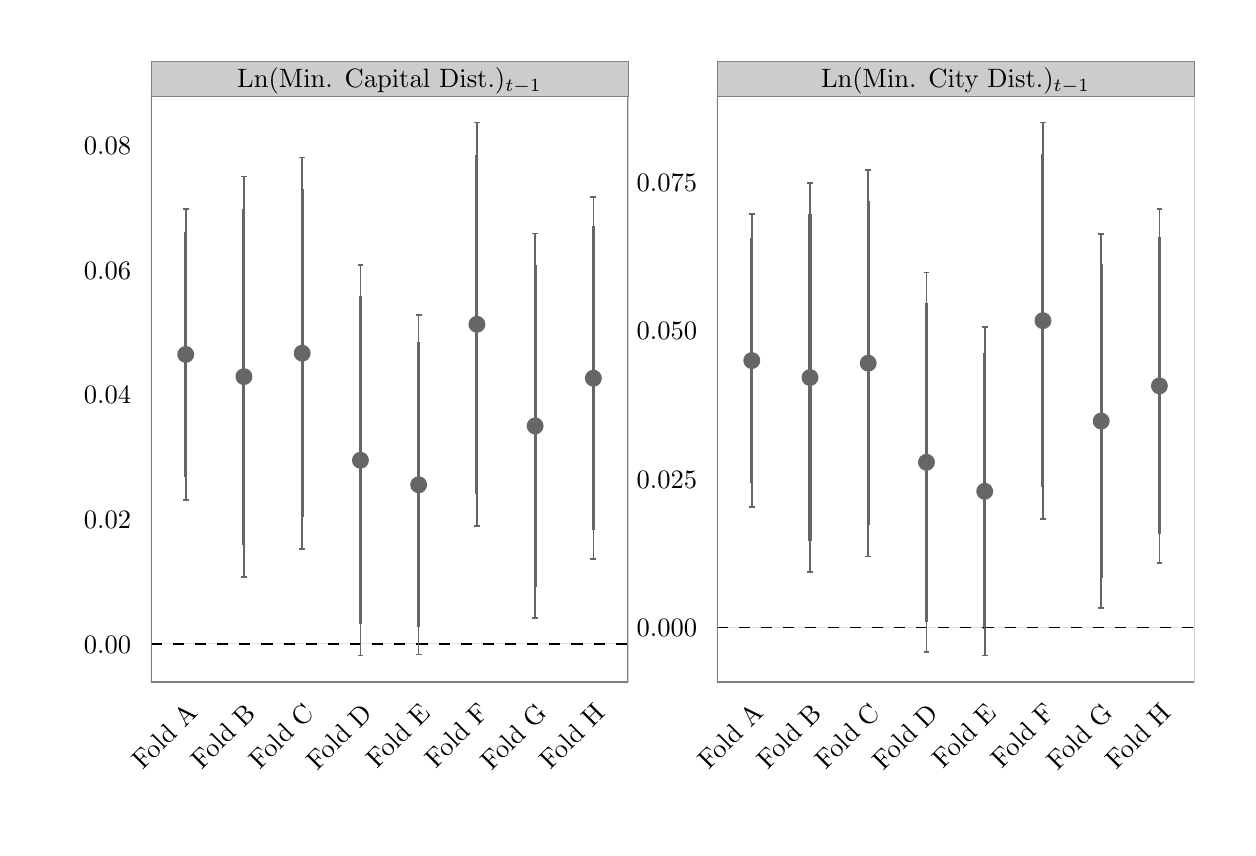
\begin{tikzpicture}[x=1pt,y=1pt]
\definecolor[named]{fillColor}{rgb}{1.00,1.00,1.00}
\path[use as bounding box,fill=fillColor,fill opacity=0.00] (0,0) rectangle (433.62,289.08);
\begin{scope}
\path[clip] (  0.00,  0.00) rectangle (433.62,289.08);
\definecolor[named]{drawColor}{rgb}{1.00,1.00,1.00}
\definecolor[named]{fillColor}{rgb}{1.00,1.00,1.00}

\path[draw=drawColor,line width= 0.6pt,line join=round,line cap=round,fill=fillColor] ( -0.00,  0.00) rectangle (433.62,289.08);
\end{scope}
\begin{scope}
\path[clip] ( 44.49, 52.60) rectangle (217.04,264.40);
\definecolor[named]{fillColor}{rgb}{1.00,1.00,1.00}

\path[fill=fillColor] ( 44.49, 52.60) rectangle (217.04,264.40);
\definecolor[named]{drawColor}{rgb}{0.40,0.40,0.40}
\definecolor[named]{fillColor}{rgb}{0.40,0.40,0.40}

\path[draw=drawColor,draw opacity=0.30,line width= 0.3pt,line join=round,fill=fillColor,fill opacity=0.30] ( 57.11,118.35) -- ( 57.11,223.64);

\path[draw=drawColor,draw opacity=0.30,line width= 0.3pt,line join=round,fill=fillColor,fill opacity=0.30] ( 78.15, 90.67) -- ( 78.15,235.31);

\path[draw=drawColor,draw opacity=0.30,line width= 0.3pt,line join=round,fill=fillColor,fill opacity=0.30] ( 99.20,100.76) -- ( 99.20,242.14);

\path[draw=drawColor,draw opacity=0.30,line width= 0.3pt,line join=round,fill=fillColor,fill opacity=0.30] (120.24, 62.23) -- (120.24,203.29);

\path[draw=drawColor,draw opacity=0.30,line width= 0.3pt,line join=round,fill=fillColor,fill opacity=0.30] (141.28, 62.56) -- (141.28,185.24);

\path[draw=drawColor,draw opacity=0.30,line width= 0.3pt,line join=round,fill=fillColor,fill opacity=0.30] (162.33,109.01) -- (162.33,254.77);

\path[draw=drawColor,draw opacity=0.30,line width= 0.3pt,line join=round,fill=fillColor,fill opacity=0.30] (183.37, 75.66) -- (183.37,214.67);

\path[draw=drawColor,draw opacity=0.30,line width= 0.3pt,line join=round,fill=fillColor,fill opacity=0.30] (204.41, 97.04) -- (204.41,227.78);
\definecolor[named]{drawColor}{rgb}{0.40,0.40,0.40}
\definecolor[named]{fillColor}{rgb}{0.40,0.40,0.40}

\path[draw=drawColor,line width= 1.1pt,line join=round,fill=fillColor] ( 57.11,126.81) -- ( 57.11,215.18);

\path[draw=drawColor,line width= 1.1pt,line join=round,fill=fillColor] ( 78.15,102.30) -- ( 78.15,223.69);

\path[draw=drawColor,line width= 1.1pt,line join=round,fill=fillColor] ( 99.20,112.12) -- ( 99.20,230.77);

\path[draw=drawColor,line width= 1.1pt,line join=round,fill=fillColor] (120.24, 73.57) -- (120.24,191.95);

\path[draw=drawColor,line width= 1.1pt,line join=round,fill=fillColor] (141.28, 72.43) -- (141.28,175.38);

\path[draw=drawColor,line width= 1.1pt,line join=round,fill=fillColor] (162.33,120.73) -- (162.33,243.06);

\path[draw=drawColor,line width= 1.1pt,line join=round,fill=fillColor] (183.37, 86.84) -- (183.37,203.49);

\path[draw=drawColor,line width= 1.1pt,line join=round,fill=fillColor] (204.41,107.55) -- (204.41,217.27);
\definecolor[named]{drawColor}{rgb}{0.00,0.00,0.00}
\definecolor[named]{fillColor}{rgb}{0.00,0.00,0.00}

\path[draw=drawColor,line width= 0.6pt,dash pattern=on 4pt off 4pt ,line join=round,fill=fillColor] ( 44.49, 66.40) -- (217.04, 66.40);
\definecolor[named]{drawColor}{rgb}{0.40,0.40,0.40}
\definecolor[named]{fillColor}{rgb}{0.40,0.40,0.40}

\path[draw=drawColor,line width= 0.4pt,line join=round,line cap=round,fill=fillColor] ( 57.11,171.00) circle (  2.85);

\path[draw=drawColor,line width= 0.4pt,line join=round,line cap=round,fill=fillColor] ( 78.15,162.99) circle (  2.85);

\path[draw=drawColor,line width= 0.4pt,line join=round,line cap=round,fill=fillColor] ( 99.20,171.45) circle (  2.85);

\path[draw=drawColor,line width= 0.4pt,line join=round,line cap=round,fill=fillColor] (120.24,132.76) circle (  2.85);

\path[draw=drawColor,line width= 0.4pt,line join=round,line cap=round,fill=fillColor] (141.28,123.90) circle (  2.85);

\path[draw=drawColor,line width= 0.4pt,line join=round,line cap=round,fill=fillColor] (162.33,181.89) circle (  2.85);

\path[draw=drawColor,line width= 0.4pt,line join=round,line cap=round,fill=fillColor] (183.37,145.16) circle (  2.85);

\path[draw=drawColor,line width= 0.4pt,line join=round,line cap=round,fill=fillColor] (204.41,162.41) circle (  2.85);

\path[draw=drawColor,line width= 0.6pt,line join=round] ( 56.06,223.64) --
	( 58.16,223.64);

\path[draw=drawColor,line width= 0.6pt,line join=round] ( 57.11,223.64) --
	( 57.11,118.35);

\path[draw=drawColor,line width= 0.6pt,line join=round] ( 56.06,118.35) --
	( 58.16,118.35);

\path[draw=drawColor,line width= 0.6pt,line join=round] ( 77.10,235.31) --
	( 79.21,235.31);

\path[draw=drawColor,line width= 0.6pt,line join=round] ( 78.15,235.31) --
	( 78.15, 90.67);

\path[draw=drawColor,line width= 0.6pt,line join=round] ( 77.10, 90.67) --
	( 79.21, 90.67);

\path[draw=drawColor,line width= 0.6pt,line join=round] ( 98.14,242.14) --
	(100.25,242.14);

\path[draw=drawColor,line width= 0.6pt,line join=round] ( 99.20,242.14) --
	( 99.20,100.76);

\path[draw=drawColor,line width= 0.6pt,line join=round] ( 98.14,100.76) --
	(100.25,100.76);

\path[draw=drawColor,line width= 0.6pt,line join=round] (119.19,203.29) --
	(121.29,203.29);

\path[draw=drawColor,line width= 0.6pt,line join=round] (120.24,203.29) --
	(120.24, 62.23);

\path[draw=drawColor,line width= 0.6pt,line join=round] (119.19, 62.23) --
	(121.29, 62.23);

\path[draw=drawColor,line width= 0.6pt,line join=round] (140.23,185.24) --
	(142.33,185.24);

\path[draw=drawColor,line width= 0.6pt,line join=round] (141.28,185.24) --
	(141.28, 62.56);

\path[draw=drawColor,line width= 0.6pt,line join=round] (140.23, 62.56) --
	(142.33, 62.56);

\path[draw=drawColor,line width= 0.6pt,line join=round] (161.27,254.77) --
	(163.38,254.77);

\path[draw=drawColor,line width= 0.6pt,line join=round] (162.33,254.77) --
	(162.33,109.01);

\path[draw=drawColor,line width= 0.6pt,line join=round] (161.27,109.01) --
	(163.38,109.01);

\path[draw=drawColor,line width= 0.6pt,line join=round] (182.32,214.67) --
	(184.42,214.67);

\path[draw=drawColor,line width= 0.6pt,line join=round] (183.37,214.67) --
	(183.37, 75.66);

\path[draw=drawColor,line width= 0.6pt,line join=round] (182.32, 75.66) --
	(184.42, 75.66);

\path[draw=drawColor,line width= 0.6pt,line join=round] (203.36,227.78) --
	(205.46,227.78);

\path[draw=drawColor,line width= 0.6pt,line join=round] (204.41,227.78) --
	(204.41, 97.04);

\path[draw=drawColor,line width= 0.6pt,line join=round] (203.36, 97.04) --
	(205.46, 97.04);
\definecolor[named]{drawColor}{rgb}{0.50,0.50,0.50}

\path[draw=drawColor,line width= 0.6pt,line join=round,line cap=round] ( 44.49, 52.60) rectangle (217.04,264.40);
\end{scope}
\begin{scope}
\path[clip] (249.02, 52.60) rectangle (421.58,264.40);
\definecolor[named]{fillColor}{rgb}{1.00,1.00,1.00}

\path[fill=fillColor] (249.02, 52.60) rectangle (421.58,264.40);
\definecolor[named]{drawColor}{rgb}{0.40,0.40,0.40}
\definecolor[named]{fillColor}{rgb}{0.40,0.40,0.40}

\path[draw=drawColor,draw opacity=0.30,line width= 0.3pt,line join=round,fill=fillColor,fill opacity=0.30] (261.65,115.91) -- (261.65,221.67);

\path[draw=drawColor,draw opacity=0.30,line width= 0.3pt,line join=round,fill=fillColor,fill opacity=0.30] (282.69, 92.41) -- (282.69,232.88);

\path[draw=drawColor,draw opacity=0.30,line width= 0.3pt,line join=round,fill=fillColor,fill opacity=0.30] (303.73, 97.96) -- (303.73,237.72);

\path[draw=drawColor,draw opacity=0.30,line width= 0.3pt,line join=round,fill=fillColor,fill opacity=0.30] (324.78, 63.40) -- (324.78,200.67);

\path[draw=drawColor,draw opacity=0.30,line width= 0.3pt,line join=round,fill=fillColor,fill opacity=0.30] (345.82, 62.23) -- (345.82,180.88);

\path[draw=drawColor,draw opacity=0.30,line width= 0.3pt,line join=round,fill=fillColor,fill opacity=0.30] (366.86,111.64) -- (366.86,254.77);

\path[draw=drawColor,draw opacity=0.30,line width= 0.3pt,line join=round,fill=fillColor,fill opacity=0.30] (387.91, 79.34) -- (387.91,214.49);

\path[draw=drawColor,draw opacity=0.30,line width= 0.3pt,line join=round,fill=fillColor,fill opacity=0.30] (408.95, 95.65) -- (408.95,223.62);
\definecolor[named]{drawColor}{rgb}{0.40,0.40,0.40}
\definecolor[named]{fillColor}{rgb}{0.40,0.40,0.40}

\path[draw=drawColor,line width= 1.1pt,line join=round,fill=fillColor] (261.65,124.41) -- (261.65,213.17);

\path[draw=drawColor,line width= 1.1pt,line join=round,fill=fillColor] (282.69,103.70) -- (282.69,221.59);

\path[draw=drawColor,line width= 1.1pt,line join=round,fill=fillColor] (303.73,109.19) -- (303.73,226.48);

\path[draw=drawColor,line width= 1.1pt,line join=round,fill=fillColor] (324.78, 74.43) -- (324.78,189.64);

\path[draw=drawColor,line width= 1.1pt,line join=round,fill=fillColor] (345.82, 71.76) -- (345.82,171.34);

\path[draw=drawColor,line width= 1.1pt,line join=round,fill=fillColor] (366.86,123.15) -- (366.86,243.27);

\path[draw=drawColor,line width= 1.1pt,line join=round,fill=fillColor] (387.91, 90.21) -- (387.91,203.63);

\path[draw=drawColor,line width= 1.1pt,line join=round,fill=fillColor] (408.95,105.94) -- (408.95,213.34);
\definecolor[named]{drawColor}{rgb}{0.00,0.00,0.00}
\definecolor[named]{fillColor}{rgb}{0.00,0.00,0.00}

\path[draw=drawColor,line width= 0.6pt,dash pattern=on 4pt off 4pt ,line join=round,fill=fillColor] (249.02, 72.38) -- (421.58, 72.38);
\definecolor[named]{drawColor}{rgb}{0.40,0.40,0.40}
\definecolor[named]{fillColor}{rgb}{0.40,0.40,0.40}

\path[draw=drawColor,line width= 0.4pt,line join=round,line cap=round,fill=fillColor] (261.65,168.79) circle (  2.85);

\path[draw=drawColor,line width= 0.4pt,line join=round,line cap=round,fill=fillColor] (282.69,162.65) circle (  2.85);

\path[draw=drawColor,line width= 0.4pt,line join=round,line cap=round,fill=fillColor] (303.73,167.84) circle (  2.85);

\path[draw=drawColor,line width= 0.4pt,line join=round,line cap=round,fill=fillColor] (324.78,132.03) circle (  2.85);

\path[draw=drawColor,line width= 0.4pt,line join=round,line cap=round,fill=fillColor] (345.82,121.55) circle (  2.85);

\path[draw=drawColor,line width= 0.4pt,line join=round,line cap=round,fill=fillColor] (366.86,183.21) circle (  2.85);

\path[draw=drawColor,line width= 0.4pt,line join=round,line cap=round,fill=fillColor] (387.91,146.92) circle (  2.85);

\path[draw=drawColor,line width= 0.4pt,line join=round,line cap=round,fill=fillColor] (408.95,159.64) circle (  2.85);

\path[draw=drawColor,line width= 0.6pt,line join=round] (260.60,221.67) --
	(262.70,221.67);

\path[draw=drawColor,line width= 0.6pt,line join=round] (261.65,221.67) --
	(261.65,115.91);

\path[draw=drawColor,line width= 0.6pt,line join=round] (260.60,115.91) --
	(262.70,115.91);

\path[draw=drawColor,line width= 0.6pt,line join=round] (281.64,232.88) --
	(283.74,232.88);

\path[draw=drawColor,line width= 0.6pt,line join=round] (282.69,232.88) --
	(282.69, 92.41);

\path[draw=drawColor,line width= 0.6pt,line join=round] (281.64, 92.41) --
	(283.74, 92.41);

\path[draw=drawColor,line width= 0.6pt,line join=round] (302.68,237.72) --
	(304.79,237.72);

\path[draw=drawColor,line width= 0.6pt,line join=round] (303.73,237.72) --
	(303.73, 97.96);

\path[draw=drawColor,line width= 0.6pt,line join=round] (302.68, 97.96) --
	(304.79, 97.96);

\path[draw=drawColor,line width= 0.6pt,line join=round] (323.73,200.67) --
	(325.83,200.67);

\path[draw=drawColor,line width= 0.6pt,line join=round] (324.78,200.67) --
	(324.78, 63.40);

\path[draw=drawColor,line width= 0.6pt,line join=round] (323.73, 63.40) --
	(325.83, 63.40);

\path[draw=drawColor,line width= 0.6pt,line join=round] (344.77,180.88) --
	(346.87,180.88);

\path[draw=drawColor,line width= 0.6pt,line join=round] (345.82,180.88) --
	(345.82, 62.23);

\path[draw=drawColor,line width= 0.6pt,line join=round] (344.77, 62.23) --
	(346.87, 62.23);

\path[draw=drawColor,line width= 0.6pt,line join=round] (365.81,254.77) --
	(367.92,254.77);

\path[draw=drawColor,line width= 0.6pt,line join=round] (366.86,254.77) --
	(366.86,111.64);

\path[draw=drawColor,line width= 0.6pt,line join=round] (365.81,111.64) --
	(367.92,111.64);

\path[draw=drawColor,line width= 0.6pt,line join=round] (386.85,214.49) --
	(388.96,214.49);

\path[draw=drawColor,line width= 0.6pt,line join=round] (387.91,214.49) --
	(387.91, 79.34);

\path[draw=drawColor,line width= 0.6pt,line join=round] (386.85, 79.34) --
	(388.96, 79.34);

\path[draw=drawColor,line width= 0.6pt,line join=round] (407.90,223.62) --
	(410.00,223.62);

\path[draw=drawColor,line width= 0.6pt,line join=round] (408.95,223.62) --
	(408.95, 95.65);

\path[draw=drawColor,line width= 0.6pt,line join=round] (407.90, 95.65) --
	(410.00, 95.65);
\definecolor[named]{drawColor}{rgb}{0.50,0.50,0.50}

\path[draw=drawColor,line width= 0.6pt,line join=round,line cap=round] (249.02, 52.60) rectangle (421.58,264.40);
\end{scope}
\begin{scope}
\path[clip] (  0.00,  0.00) rectangle (433.62,289.08);
\definecolor[named]{drawColor}{rgb}{0.50,0.50,0.50}
\definecolor[named]{fillColor}{rgb}{0.80,0.80,0.80}

\path[draw=drawColor,line width= 0.2pt,line join=round,line cap=round,fill=fillColor] ( 44.49,264.40) rectangle (217.04,277.04);
\definecolor[named]{drawColor}{rgb}{0.00,0.00,0.00}

\node[text=drawColor,anchor=base,inner sep=0pt, outer sep=0pt, scale=  0.96] at (130.76,267.41) {Ln(Min. Capital Dist.)$_{t-1}$};
\end{scope}
\begin{scope}
\path[clip] (  0.00,  0.00) rectangle (433.62,289.08);
\definecolor[named]{drawColor}{rgb}{0.50,0.50,0.50}
\definecolor[named]{fillColor}{rgb}{0.80,0.80,0.80}

\path[draw=drawColor,line width= 0.2pt,line join=round,line cap=round,fill=fillColor] (249.02,264.40) rectangle (421.58,277.04);
\definecolor[named]{drawColor}{rgb}{0.00,0.00,0.00}

\node[text=drawColor,anchor=base,inner sep=0pt, outer sep=0pt, scale=  0.96] at (335.30,267.41) {Ln(Min. City Dist.)$_{t-1}$};
\end{scope}
\begin{scope}
\path[clip] (  0.00,  0.00) rectangle (433.62,289.08);
\definecolor[named]{drawColor}{rgb}{0.00,0.00,0.00}

\node[text=drawColor,anchor=base east,inner sep=0pt, outer sep=0pt, scale=  0.96] at ( 37.37, 63.09) {0.00};

\node[text=drawColor,anchor=base east,inner sep=0pt, outer sep=0pt, scale=  0.96] at ( 37.37,108.14) {0.02};

\node[text=drawColor,anchor=base east,inner sep=0pt, outer sep=0pt, scale=  0.96] at ( 37.37,153.18) {0.04};

\node[text=drawColor,anchor=base east,inner sep=0pt, outer sep=0pt, scale=  0.96] at ( 37.37,198.23) {0.06};

\node[text=drawColor,anchor=base east,inner sep=0pt, outer sep=0pt, scale=  0.96] at ( 37.37,243.28) {0.08};
\end{scope}
\begin{scope}
\path[clip] (  0.00,  0.00) rectangle (433.62,289.08);
\definecolor[named]{drawColor}{rgb}{0.00,0.00,0.00}

\node[text=drawColor,anchor=base east,inner sep=0pt, outer sep=0pt, scale=  0.96] at (241.91, 69.07) {0.000};

\node[text=drawColor,anchor=base east,inner sep=0pt, outer sep=0pt, scale=  0.96] at (241.91,122.66) {0.025};

\node[text=drawColor,anchor=base east,inner sep=0pt, outer sep=0pt, scale=  0.96] at (241.91,176.25) {0.050};

\node[text=drawColor,anchor=base east,inner sep=0pt, outer sep=0pt, scale=  0.96] at (241.91,229.84) {0.075};
\end{scope}
\begin{scope}
\path[clip] (  0.00,  0.00) rectangle (433.62,289.08);
\definecolor[named]{drawColor}{rgb}{0.00,0.00,0.00}

\node[text=drawColor,rotate= 45.00,anchor=base east,inner sep=0pt, outer sep=0pt, scale=  0.96] at ( 61.79, 40.81) {Fold A};

\node[text=drawColor,rotate= 45.00,anchor=base east,inner sep=0pt, outer sep=0pt, scale=  0.96] at ( 82.83, 40.81) {Fold B};

\node[text=drawColor,rotate= 45.00,anchor=base east,inner sep=0pt, outer sep=0pt, scale=  0.96] at (103.87, 40.81) {Fold C};

\node[text=drawColor,rotate= 45.00,anchor=base east,inner sep=0pt, outer sep=0pt, scale=  0.96] at (124.92, 40.81) {Fold D};

\node[text=drawColor,rotate= 45.00,anchor=base east,inner sep=0pt, outer sep=0pt, scale=  0.96] at (145.96, 40.81) {Fold E};

\node[text=drawColor,rotate= 45.00,anchor=base east,inner sep=0pt, outer sep=0pt, scale=  0.96] at (167.00, 40.81) {Fold F};

\node[text=drawColor,rotate= 45.00,anchor=base east,inner sep=0pt, outer sep=0pt, scale=  0.96] at (188.04, 40.81) {Fold G};

\node[text=drawColor,rotate= 45.00,anchor=base east,inner sep=0pt, outer sep=0pt, scale=  0.96] at (209.09, 40.81) {Fold H};
\end{scope}
\begin{scope}
\path[clip] (  0.00,  0.00) rectangle (433.62,289.08);
\definecolor[named]{drawColor}{rgb}{0.00,0.00,0.00}

\node[text=drawColor,rotate= 45.00,anchor=base east,inner sep=0pt, outer sep=0pt, scale=  0.96] at (266.32, 40.81) {Fold A};

\node[text=drawColor,rotate= 45.00,anchor=base east,inner sep=0pt, outer sep=0pt, scale=  0.96] at (287.37, 40.81) {Fold B};

\node[text=drawColor,rotate= 45.00,anchor=base east,inner sep=0pt, outer sep=0pt, scale=  0.96] at (308.41, 40.81) {Fold C};

\node[text=drawColor,rotate= 45.00,anchor=base east,inner sep=0pt, outer sep=0pt, scale=  0.96] at (329.45, 40.81) {Fold D};

\node[text=drawColor,rotate= 45.00,anchor=base east,inner sep=0pt, outer sep=0pt, scale=  0.96] at (350.50, 40.81) {Fold E};

\node[text=drawColor,rotate= 45.00,anchor=base east,inner sep=0pt, outer sep=0pt, scale=  0.96] at (371.54, 40.81) {Fold F};

\node[text=drawColor,rotate= 45.00,anchor=base east,inner sep=0pt, outer sep=0pt, scale=  0.96] at (392.58, 40.81) {Fold G};

\node[text=drawColor,rotate= 45.00,anchor=base east,inner sep=0pt, outer sep=0pt, scale=  0.96] at (413.62, 40.81) {Fold H};
\end{scope}
\end{tikzpicture}
